%%%%%%%%%%%%%%%%%%%%%%%%%%%%%%%%%%%%%%%%%
% Masters/Doctoral Thesis 
% LaTeX Template
% Version 2.4 (22/11/16)
%
% This template has been downloaded from:
% http://www.LaTeXTemplates.com
%
% Version 2.x major modifications by:
% Vel (vel@latextemplates.com)
%
% This template is based on a template by:
% Steve Gunn (http://users.ecs.soton.ac.uk/srg/softwaretools/document/templates/)
% Sunil Patel (http://www.sunilpatel.co.uk/thesis-template/)
%
% Template license:
% CC BY-NC-SA 3.0 (http://creativecommons.org/licenses/by-nc-sa/3.0/)
%
%%%%%%%%%%%%%%%%%%%%%%%%%%%%%%%%%%%%%%%%%

%----------------------------------------------------------------------------------------
%	PACKAGES AND OTHER DOCUMENT CONFIGURATIONS
%----------------------------------------------------------------------------------------

\documentclass[
11pt, % The default document font size, options: 10pt, 11pt, 12pt
%oneside, % Two side (alternating margins) for binding by default, uncomment to switch to one side
% english, % ngerman for German
spanish,
singlespacing, % Single line spacing, alternatives: onehalfspacing or doublespacing
%draft, % Uncomment to enable draft mode (no pictures, no links, overfull hboxes indicated)
%nolistspacing, % If the document is onehalfspacing or doublespacing, uncomment this to set spacing in lists to single
%liststotoc, % Uncomment to add the list of figures/tables/etc to the table of contents
%toctotoc, % Uncomment to add the main table of contents to the table of contents
%parskip, % Uncomment to add space between paragraphs
%nohyperref, % Uncomment to not load the hyperref package
headsepline, % Uncomment to get a line under the header
%chapterinoneline, % Uncomment to place the chapter title next to the number on one line
%consistentlayout, % Uncomment to change the layout of the declaration, abstract and acknowledgements pages to match the default layout
]{MastersDoctoralThesis} % The class file specifying the document structure

\usepackage[utf8]{inputenc} % Required for inputting international characters
\usepackage[T1]{fontenc} % Output font encoding for international characters

\usepackage{palatino} % Use the Palatino font by default

\usepackage[nottoc]{tocbibind} %Paquete para incluir la bibliografía en el índice
% \usepackage[autostyle=true]{csquotes} % Required to generate language-dependent quotes in the bibliography


% \usepackage[backend=bibtex,style=alphabetic,natbib=true]{biblatex} % Use the bibtex backend with the authoryear citation style (which resembles APA)
% \addbibresource{bib.bib} % The filename of the bibliography

\usepackage{csvsimple}
\usepackage{xcolor}

\usepackage{enumitem}
\setlist[enumerate]{label*=\arabic*.}

\usepackage[square,numbers]{natbib}
\bibliographystyle{abbrvnat}
\setcitestyle{authoryear,open={(},close={)}}
% \citep{biopac}

\usepackage{amsmath}
% \usepackage[spanish,onelanguage,ruled]{algorithm2e} % for algorithm pseudocode
\usepackage[ruled]{algorithm2e} % for algorithm pseudocode

% Please add the following required packages to your document preamble:
\usepackage{booktabs}

% \usepackage[spanish, es-tabla]{babel}

%----------------------------------------------------------------------------------------
%	MARGIN SETTINGS
%----------------------------------------------------------------------------------------

\geometry{
	paper=a4paper, % Change to letterpaper for US letter
	inner=1.8cm, % Inner margin
	outer=3.1cm, % Outer margin
	bindingoffset=.5cm, % Binding offset
	top=1.5cm, % Top margin
	bottom=1.5cm, % Bottom margin
	%showframe, % Uncomment to show how the type block is set on the page
}

%----------------------------------------------------------------------------------------
%	THESIS INFORMATION
%----------------------------------------------------------------------------------------

\thesistitle{Análisis de productos químicos \\ en cosméticos} % Your thesis title, this is used in the title and abstract, print it elsewhere with \ttitle
\supervisor{Juan Manuel \\ \textsc{Moreno Lamparero}} % Your supervisor's name, this is used in the title page, print it elsewhere with \supname
\examiner{} % Your examiner's name, this is not currently used anywhere in the template, print it elsewhere with \examname
\degree{Máster en \\ Big Data \& Business Analytics} % Your degree name, this is used in the title page and abstract, print it elsewhere with \degreename
\author{José María \\ \textsc{Sánchez Salas}} % Your name, this is used in the title page and abstract, print it elsewhere with \authorname
% \newcommand{\mention}{Mención: Computación}
\addresses{} % Your address, this is not currently used anywhere in the template, print it elsewhere with \addressname

% \subject{Biological Sciences} % Your subject area, this is not currently used anywhere in the template, print it elsewhere with \subjectname
\keywords{} % Keywords for your thesis, this is not currently used anywhere in the template, print it elsewhere with \keywordnames
\university{IMF Business School \\ Universidad Camilo José Cela} % Your university's name and URL, this is used in the title page and abstract, print it elsewhere with \univname
% \department{\href{http://www.um.es/web/diic/}{Departamento de Ingeniería de la Información y las Comunicaciones}} % Your department's name and URL, this is used in the title page and abstract, print it elsewhere with \deptname
% \group{\href{http://researchgroup.university.com}{Research Group Name}} % Your research group's name and URL, this is used in the title page, print it elsewhere with \groupname
% \faculty{\href{http://www.um.es/informatica}{Facultad de Informática}} % Your faculty's name and URL, this is used in the title page and abstract, print it elsewhere with \facname

\AtBeginDocument{
\hypersetup{pdftitle=\ttitle} % Set the PDF's title to your title
\hypersetup{pdfauthor=\authorname} % Set the PDF's author to your name
\hypersetup{pdfkeywords=\keywordnames} % Set the PDF's keywords to your keywords
}

\usepackage{hyperref}


\setcounter{secnumdepth}{3} % Para enumerar hasta subsubsection
\setcounter{tocdepth}{2} % Para enumerar hasta subsection 

\begin{document}

\nocite{*} % For show all references which are not cited

\frontmatter % Use roman page numbering style (i, ii, iii, iv...) for the pre-content pages

\pagestyle{plain} % Default to the plain heading style until the thesis style is called for the body content

%----------------------------------------------------------------------------------------
%	TITLE PAGE
%----------------------------------------------------------------------------------------

\begin{titlepage}
\begin{center}

\vspace*{.06\textheight}
{\scshape\LARGE \univname\par}\vspace{1.5cm} % University name
\vspace{10mm}% \includegraphics[scale=0.7]{umu-logo}\\\vspace{1cm} 
{\scshape\huge \degreename\par} \vspace{1.5cm} % Degree name 
% {\scshape\Large \mention\par}\vspace{1cm} % Mention name
\textsc{\LARGE Trabajo Fin de Máster}\\[0.5cm] % Thesis type

\vspace{10mm}
\HRule \\[0.4cm] % Horizontal line
{\huge \bfseries \ttitle\par}\vspace{0.4cm} % Thesis title
\HRule \\[2.5cm] % Horizontal line
 
\begin{minipage}[t]{0.4\textwidth}
\begin{flushleft} \large
\emph{Autor:}\\
\authorname % Author name - remove the \href bracket to remove the link
\end{flushleft}
\end{minipage}
\begin{minipage}[t]{0.4\textwidth}
\begin{flushright} \large
\emph{Tutor:} \\
\supname % Supervisor name - remove the \href bracket to remove the link  
\end{flushright}
\end{minipage}\\[1.5cm]
 
\vfill

{\large \textsc{Marzo 2019}}\\[4cm] % Date
 
\vfill
\end{center}
\end{titlepage}

\cleardoublepage

%----------------------------------------------------------------------------------------
%	QUOTATION PAGE
%----------------------------------------------------------------------------------------

\vspace*{0.2\textheight}

\noindent{\itshape Una de las cosas más fascinantes de los programadores es que no puedes saber si están trabajando o no sólo con mirarlos. A menudo están sentados aparentemente tomando café, chismorreando o mirando a las nubes. Sin embargo, es posible que estén poniendo en orden todas las ideas individuales y sin relación que pululan por su mente.}\bigbreak

\hfill Charles M. Strauss

\newpage
\cleardoublepage
\newpage

\vspace*{0.2\textheight}

\begin{flushright}
 
\noindent{\itshape Como dirían en el cole: \\ no hay mejor consejo que el de ser tú mismo, \\ a pesar de que al resto no les mole.}\bigbreak

\hfill ZPU

\end{flushright}


%----------------------------------------------------------------------------------------
%	ACKNOWLEDGEMENTS
%----------------------------------------------------------------------------------------

\begin{acknowledgements}
\addchaptertocentry{\acknowledgementname} % Add the acknowledgements to the table of contents
% 

Mi más sincero agradecimiento a mi tutor Juan Manuel Moreno Lamparero, por abrirme las puertas a un sin fin de posibilidades, por todo su apoyo y dedicación durante todo este tiempo. \\

Al kárate, por seguir siendo el eje central. A mi nueva familia del Gimnasio Noru, por abrirme sus puertas y recibirme como uno más. A Javier Domínguez, allá donde esté, por haber formado esa gran familia y por haberme transmitido tanto en tan poco tiempo. ¿Dragón o Tigre? \\

A mis amigos Miki, Negro y Wawas por seguir permaneciendo a mi lado a pesar de la distancia. A mi amiga Miriam, por hacer que te sienta tan cerca estando cada vez más lejos. \\

A mis amigos de Madrid. A Sara. A Vero, Cristina, Cristian y Víctor. A Borja. A Sergio Alcalde. Por haberme acompañado en esta etapa de mi vida, que se cierra en breve. \\

A mis padres, Juan y Carmen, y a mi hermano Juan Luis, por su apoyo y amor incondicional desde la distancia. Por su fe ciega en mí. 

\end{acknowledgements}


%----------------------------------------------------------------------------------------
%	ABSTRACT PAGE
%----------------------------------------------------------------------------------------

\begin{abstract}
\addchaptertocentry{\abstractname} % Add the abstract to the table of contents
% En este Trabajo Fin de Grado (\gls{TFG}) se expone el diseño e implementación de una herramienta web para el análisis, procesamiento y visualización de señales del electroencefalograma (\gls{EEG}). Este trabajo es la continuación del \gls{TFG}: \textit{Análisis de \gls{EEG} para la evaluación de las emociones} \cite{tesis-hugo}, en el que se describen las técnicas y procedimientos para el procesamiento y análisis de señales del \gls{EEG}, y que está implementado completamente en Matlab. \\

El objetivo principal subyacente a la realización de este trabajo es la obtención de una herramienta de \textit{software libre} que permita el cálculo de medidas objetivas a partir del procesamiento del electroencefalograma. En este trabajo, las medidas objetivas son los siguientes cuatro índices: \textit{Índice de atención, Índice de memorización, Índice de aproximación-rechazo e Índice de compromiso}. \\

Además, otro de los objetivos de este trabajo es que la herramienta proporcione la visualización de todas las señales y de todos los valores intermedios que se utilizan en todas las fases del cálculo de estos índices.\\

Esta herramienta web está implementada completamente en el entorno matemático R, tanto la parte del servidor \textit{(backend)} como la parte de interfaz de usuario \textit{(frontend)}. Para ello se ha hecho uso del framework web Shiny. \\

Para la obtención de los índices, el primer problema planteado es el entendimiento e interiorización de todo el \gls{TFG} \cite{tesis-hugo}, desde los conceptos médicos del \gls{EEG} hasta el cálculo final de los índices. El segundo problema consiste en aprender el framework Shiny, sus características y cómo funciona para poder realizar la implementación de la herramienta. \\

El tercero es estudiar y analizar distintas técnicas de filtrado de señales, así como distintas herramientas para la visualización de las mismas. El cuarto problema es realizar la implementación de todo el procedimiento para el cálculo de los índices. Y por último, realizar una evaluación de los resultados obtenidos en comparación con los obtenidos en \cite{tesis-hugo}.



\end{abstract}


%----------------------------------------------------------------------------------------
%	LIST OF CONTENTS/FIGURES/TABLES PAGES
%----------------------------------------------------------------------------------------

\tableofcontents % Prints the main table of contents

\renewcommand{\listfigurename}{Índice de figuras}
\renewcommand{\figurename}{Figura}

\listoffigures % Prints the list of figures

\renewcommand{\listtablename}{Índice de tablas}
\renewcommand{\tablename}{Tabla}

\listoftables % Prints the list of tables

%----------------------------------------------------------------------------------------
% Define some commands to keep the formatting separated from the content 
\newcommand{\keyword}[1]{\textbf{#1}}
\newcommand{\tabhead}[1]{\textbf{#1}}
\newcommand{\code}[1]{\texttt{#1}}
\newcommand{\file}[1]{\texttt{\bfseries#1}}
\newcommand{\option}[1]{\texttt{\itshape#1}}
%----------------------------------------------------------------------------------------

\mainmatter % Begin numeric (1,2,3...) page numbering

\pagestyle{thesis} % Return the page headers back to the "thesis" style

% Include the chapters of the thesis as separate files from the Chapters folder
% Uncomment the lines as you write the chapters

% Chapter Template

\chapter{Introducción y antecedentes} % Main chapter title
\label{chap:introduction} % Change X to a consecutive number; for referencing this chapter elsewhere, use \ref{ChapterX}

%------------------------------------------------
\section{Introducción}

La preocupación del ser humano por su aspecto y su cuidado es algo que se ha ido manteniendo a lo largo de los siglos, pues aunque hoy en día la industria cosmética parezca algo tecnológico y sofisticado, las primeras civilizaciones ya se preocupaban por ello. Precisamente, en el Antiguo Egipto se encuentran los primeros vestigios de la elaboración y utilización de diferentes productos cosméticos, utilizando para ello productos naturales, como plantas aromáticas. \\

La cosmética es uno de los sectores que mayor auge ha vivido durante las últimas décadas. Entre los siglos XVI al XVIII se produjo un gran desarrollo de los cosméticos y se introdujeron numerosos productos nuevos, aún fabricados principalmente a base de plantas. Pero fue a partir de principios del siglo XX cuando los cosméticos se popularizarían, hasta convertirse hoy en un producto casi imprescindible en la mayoría de los hogares. \\

Hoy en día, los cosméticos han vuelto a incorporar productos químicos dentro de sus fórmulas y se utilizan miles de estos compuestos a los que se le atribuyen multitud de propiedades. Sin embargo, varios cientificos y organizaciones han levantado la voz de alerta sobre el impacto de estos compuestos, pues en un alto porcentaje no han sido analizados para saber el daño de estos productos sobre las personas.



%------------------------------------------------
\section{Antecedentes}

Este trabajo se embarca dentro del contexto de la aplicación de técnicas Big Data e Inteligencia Artificial al sector de la cosmética. Existen varios productos y prototipos de productos que aplican al sector cosmético este tipo de técnicas, como por ejemplo el servicio \href{https://rewisor.com/la-ia-y-el-big-data-llegan-pisando-fuerte-al-mundo-de-la-cosmetica/}{\color{blue}{\underline{Identité}}}, que utiliza técnicas de Inteligencia Artificial y Big Data para ``Crear paquetes de belleza y productos para el cuidado de la piel muy personalizados.''. 





%------------------------------------------------
\section{Estructura de la memoria}



















% Chapter Template

\chapter{Hipótesis de trabajo y objetivos} % Main chapter title
\label{chap:job-hypothesis} % Change X to a consecutive number; for referencing this chapter elsewhere, use \ref{ChapterX}


%------------------------------------------------    
\section{Introducción}
En este capítulo se va a exponer la hipótesis de este trabajo así como los objetivos propuestos para el mismo.



%------------------------------------------------    
\section{Hipótesis de trabajo}

Los cosméticos son unos de los productos que más se consumen en los hogares, hasta tal punto que en algunos casos se han vuelto imprescindibles. Muchos productos químicos diferentes se utilizan en la fabricación de cosméticos. Los grupos de defensa de consumidores y trabajadores están preocupados porque algunos productos cosméticos contienen sustancias químicas que se sabe o se sospecha que causan cáncer, defectos de nacimiento o daños al sistema reproductivo. Aquellos que trabajan con cosméticos, incluidos los peluqueros, los estilistas y el cuidado de la piel, el cuidado del cuerpo y los trabajadores de salones de uñas, pueden ser más vulnerables a los efectos adversos para la salud que presentan estos productos porque manejan con mayor frecuencia grandes cantidades de cosméticos \citep{dataset}. \\

Con esta idea en mente, la hipótesis de este trabajo es aplicar técnicas de Inteligencia Artificial y Big Data al sector de la cosmética para poder encontrar patrones y relaciones entre los cosméticos y los productos químicos que contienen, así como encontrar una clasificación de dichos productos químicos para poder tener un mayor control sobre de qué están compuestos los cosméticos que consumimos. \\




%------------------------------------------------    
\section{Objetivos}
\label{sec:goals}

Los objetivos principales de este trabajo son:
\begin{itemize}
 \item Encontrar una clasificación de los productos químicos presentes en los cosméticos.
 \item Encontrar qué productos químicos son los más frecuentes en los cosméticos, así como los cosméticos que mayor productos químicos presentan.
 \item Obtener una predicción de la cantidad de productos químicos dañinos que contendrán los futuros cosméticos.
\end{itemize}

























% Chapter Template

\chapter{Material y métodos} % Main chapter title
\label{chap:material-methods} % Change X to a consecutive number; for referencing this chapter elsewhere, use \ref{ChapterX}


%------------------------------------------------    
\section{Introducción}

En este capítulo se detallará, en primer lugar, el dataset utilizado para el desarrollo de este trabajo, la descripción de sus características y la selección de las características más importantes. En segundo lugar, se detallarán los métodos y técnicas que se han aplicado al dataset para conseguir los objetivos de este trabajo.





%------------------------------------------------    
\section{Material}
\label{sec:material}

Para la realización de este trabajo se ha hecho uso del dataset público \tabhead{Chemicals in Cosmetics} \citep{dataset} proporcionado por \tabhead{HealthData} \citep{healthdata}. \\

Para todos los productos cosméticos vendidos en California, la Ley de Cosméticos Seguros de California requiere que el fabricante, empacador y/o distribuidor nombrado en la etiqueta del producto proporcione una lista al Programa de Cosméticos Seguros de California \textit{(California Safe Cosmetics Program (CSCP))} perteneciente al Departamento de Salud Pública de California \textit{(California Department of Public Health (CDPH))} de todos los productos cosméticos que contengan cualquier ingrediente conocido o sospechoso de causar cáncer, defectos de nacimiento u otros daños al desarrollo o reproductivos. El CSCP mantiene una lista de ingredientes ``reportables''. Las compañías con ingredientes reportables en sus productos deben enviar información al Programa de Cosméticos Seguros de California si la compañía:

\begin{itemize}
 \item Tiene ventas anuales agregadas de productos cosméticos de un millón de dólares o más, y
 \item Ha vendido productos cosméticos en California a partir del 1 de enero de 2007.
\end{itemize}

El CSCP mantiene un sistema de informes \textit{online} para que las empresas informen sobre productos e ingredientes reportables, generando así el dataset utilizado para este trabajo. Los datos reflejan información que ha sido reportada al CSCP. No se incluyen todos los productos que contengan carcinógenos o tóxicos para el desarrollo o la reproducción, debido a que las compañías no los informan.



%------------------------------------------------    
\subsection{Descripción del dataset}
\label{sec:dataset-description}

El dataset proporcionado por el CSCP es un dataset en formato CSV con un histórico desde el año 2009 y que se va actualizando cada 3 o 4 días. En las fechas de realización de este trabajo (última fecha reportada: 21/02/2019), el dataset consta de:

\begin{itemize}
 \item 97.760 registros.
 \item 22 columnas (características).
\end{itemize}

En la Tabla \ref{tab:features} se describen cada una de las características. La agrupación de las características \code{CDPHId}, \code{CSFId}, \code{SubCategoryId} y \code{ChemicalId} forma la clave primaria de este dataset.


%------------------------------------------------    
\subsection{Selección de características importantes}

No todas las características descritas en la Tabla \ref{tab:features} son necesarias para aplicar las técnicas descritas en la sección \ref{sec:methods} ya que algunas de ellas son informativas o no son relevantes a la hora de aplicar dichas técnicas. \\

Se van a tener en cuenta todas las características de formato Fecha, exceptuando las características \code{DiscontinuedDate} y \code{ChemicalDateRemoved}, ya que solamente interesan aquellos productos que no hayan sido eliminados. Además, se van a utilizar las características \code{SubCategoryId} y \code{CASId}, pues son los identificadores de los cosméticos y los productos químicos, respectivamente. Se utiliza \code{SubCategoryId} en vez de \code{PrimaryCategoryId} debido a que la primera es más específica que la segunda y a partir de la primera se puede sacar la segunda (pues está contenido en ella). Y por supuesto, \code{ChemicalCount}, que indica la cantidad de productos químicos. \\

Así pues, la Tabla \ref{tab:features-selection} muestra las características que se van a tener en cuenta:

\begin{table}[!th]
\begin{tabular}{@{}l@{}}
\toprule
Nombre                         \\ \midrule
\code{SubCategoryId}           \\
\code{CASId}                   \\
\code{InitialDateReported}     \\
\code{MostRecentDateReported}  \\ 
\code{ChemicalCreatedAt}       \\
\code{ChemicalUpdatedAt}       \\ 
\code{ChemicalCount}           \\
\bottomrule
\end{tabular}
\centering
\caption{Selección de características importantes.}
\label{tab:features-selection}
\end{table}



\begin{table}[]
\begin{tabular}{@{}lll@{}}
\toprule
Nombre                 & Formato & Definición \\ \midrule
\code{CDPHId}          & Texto & Número identificativo interno del CDPH \\ & & para el producto. \\
\code{ProductName}     & Texto & Nombre del producto introducido por \\ & & el fabricante, empacador y/o distribuidor. \\
\code{CSFId}           & Texto & Número identificativo interno del CDPH \\ & & para el color/aroma/sabor. \\
\code{CSF}             & Texto & Color, aroma y/o sabor introducido por \\ & & el fabricante, empacador y/o distribuidor. \\                                                                                                                                             
\code{CompanyId}       & Texto & Número identificativo interno del CDPH \\ & & para la compañía. \\
\code{CompanyName}     & Texto & Nombre de la compañía introducido por \\ & & el fabricante, empacador y/o distribuidor. \\
\code{BrandName}       & Texto & Nombre de la marca introducido por \\ & & el fabricante, empacador y/o distribuidor. \\
\code{PrimaryCategoryId}  & Texto & Número identificativo interno del CDPH \\ & & para la categoría. \\
\code{PrimaryCategory}    & Texto & Tipo de producto (13 categorías primarias). \\
\code{SubCategoryId}      & Texto & Número identificativo interno del CDPH \\ & & para la subcategoría. \\
\code{SubCategory}        & Texto & Tipo de producto dentro de una de las \\ & & categorías primarias. \\
\code{CASId}              & Texto & Número identificativo interno del CDPH \\ & & para el producto químico. \\
\code{CasNumber}          & Texto & Número identificativo del producto \\ & & químico seleccionado por el fabricante, \\ & & empacador y/o distribuidor. \\ 
\code{ChemicalId}         & Texto & Número identificativo interno del CDPH \\ & & para el registro específico del producto \\ & & químico en ese cosmético. \\
\code{ChemicalName}       & Texto & Nombre del producto químico \\ & & seleccionado por el fabricante, empacador \\ & & y/o distribuidor. \\ 
\code{InitialDateReported}     & Fecha & Fecha en la que el cosmético fue \\ & & reportado por primera vez al CDPH. \\
\code{MostRecentDateReported}  & Fecha & Fecha de la última modificación del perfil \\ & & del cosmético por el fabricante, \\ & & empacador y/o distribuidor. \\ 
\code{DiscontinuedDate}        & Fecha & Si aplica, fecha en la que el cosmético fue \\ & & interrumpido. \\ 
\code{ChemicalCreatedAt}       & Fecha & Fecha en la que el producto químico fue \\ & & reportado al CDPH por primera vez en \\ & & ese cosmético. \\
\code{ChemicalUpdatedAt}       & Fecha & Fecha de la última modificación del perfil \\ & & del producto químico por el fabricante, \\ & & empacador y/o distribuidor. \\ 
\code{ChemicalDateRemoved}     & Fecha & Si aplica, fecha en la que el producto \\ & & químico fue eliminado del cosmético. \\ 
\code{ChemicalCount}           & Número & Número total de productos químicos \\ & &  reportados en ese cosmético \\
\bottomrule
\end{tabular}
\centering
\caption{Descripción de las características del dataset.}
\label{tab:features}
\end{table}


\newpage
%------------------------------------------------    
\section{Métodos}
\label{sec:methods}

Este trabajo se va a realizar utilizando el lenguaje de programación Python y como entorno de desarrollo Jupyter Notebook. Los métodos que se van a utilizar para la consecución de los objetivos descritos en la sección \ref{sec:goals} son:


%------------------------------------------------    
\subsection{Obtención del dataset}

Como se ha comentado en la sección \ref{sec:material}, el dataset se haya ubicado en la plataforma HealthData y además es incremental \citep{dataset}, por lo que para obtener dicho dataset se va a hacer uso de la API \citep{healthdata-api} que proporciona HealhData. \\



%------------------------------------------------    
\subsection{Clustering}

Para poder obtener la clasificación de los productos químicos presentes en los cosméticos, se van a aplicar técnicas de Clustering. Concretamente, se va a utilizar la implementación del algoritmo K-Means proporcionada por Scikit-learn \citep{scikit-learn}.



%------------------------------------------------    
\subsection{Data Analysis}

Para poder encontrar qué productos químicos son más frecuentes, así como aquellos cosméticos que presentan mayor número de productos químicos, se van a aplicar técnicas de Data Science como el Análisis Exploratorio de Datos \textit{(Exploratory Data Analysis (EDA))} \citep{eda}. La aplicación de EDA se va a realizar haciendo uso de los resultados obtenidos tras la clusterización.


%------------------------------------------------    
\subsection{Forecasting}

Para poder obtener la predicción de la cantidad de productos químicos que contendrán los futuros cosméticos, se van a aplicar técnicas de Forecasting. Concretamente, se va a utilizar la implementación del modelo ARIMA proporcionada por StatsModels \citep{arima}.




 
% Chapter Template

\chapter{Aplicación de Técnicas y Resultados} % Main chapter title
\label{chap:results} % Change X to a consecutive number; for referencing this chapter elsewhere, use \ref{ChapterX}


%------------------------------------------------   
\section{Introducción}

En este capítulo se realizará la explicación de todas las técnicas aplicadas sobre el dataset. En primer lugar, se detallará cómo se ha realizado la obtención del dataset; en segundo lugar, cómo se ha realizado la aplicación de las técnicas de clustering; en tercer lugar, los resultados obtenidos tras la aplicación del análisis exploratorio de los datos; y en último lugar, cómo se ha realizado la aplicación de las técnicas de forecasting. \\

El código asociado a este capítulo se encuentra en el repositorio público \citep{master}.



%------------------------------------------------   
\section{Obtención del dataset}
\label{sec:data-downloading}

El dataset empleado para este trabajo es un dataset incremental actualizado cada 3 o 4 días, por lo que solo sería necesario descargar el dataset cuando haya sido actualizado. Sin embargo, el volumen de registros añadidos en cada actualización no son significativos para la aplicación de las técnicas de clustering y forecasting, de tal manera que la descarga de los datos se realiza si han pasado, como mínimo, 15 días desde la última descarga del dataset (el número de días es un parámetro configurable). Así, cada vez que se descarga el dataset, el volumen de registros nuevos que sí es significativo para la aplicación de las técnicas de clustering y forecasting. \\

El dataset en formato CSV se almacena dentro de la carpeta \code{src/data/} mientras que la información que viene asociada \citep{dataset} se almacena en la carpeta \\ \code{src/data/info/}. Por último, junto al dataset se almacena el fichero \code{local\_data\_date} con la marca de tiempo en el que se descargó el dataset. Cada vez que se descarga el dataset, el antiguo dataset (y su información asociada) queda almacenado en la carpeta \\ \code{src/data\_backup/}. \\

Todo esto se encuentra implementado en el notebook \code{src/download\_data.ipynb} \citep{master}.


%------------------------------------------------   
\section{Clustering}
\label{sec:results-clustering}

La aplicación de técnicas de clustering permite obtener agrupaciones y relaciones en los datos que a simple vista no se pueden obtener. En esta sección se va a realizar la aplicación del algoritmo de clustering K-Means \citep{scikit-learn}, realizando primero un preprocesamiento de los datos y posteriormente la obtención de algunas métricas sobre los clusters obtenidos. Todo esto se encuentra implementado en el notebook \\ \code{src/clustering-and-data-analysis.ipynb} \citep{master}.


%------------------------------------------------   
\subsection{Preprocesamiento}
\label{sec:clustering-preprocessing}

Antes de poder aplicar el algoritmo de clustering K-Means \citep{scikit-learn}, el dataset debe ser preprocesado. El preprocesamiento de este dataset ha consistido en los siguientes pasos:

\begin{itemize}
 \item \textbf{Rellenar valores nulos}. En el dataset se han encontrado tres tipos de valores nulos: 
 \begin{itemize}
  \item \textbf{Valores de formato fecha}. Han sido rellenados con el valor \code{01/01/1990}.
  \item \textbf{Valores de formato texto}. Han sido rellenados con el valor de la cadena vacía.
  \item \textbf{Valores de formato texto asociados a identificadores}. Han sido rellenados con el valor \code{-1}.
 \end{itemize}
 
 \item \textbf{Eliminar de los registros} con valor distinto de \code{01/01/1990} en los campos \\ \code{DiscontinuedDate} y \code{ChemicalDateRemoved}, pues solo se precisan de aquellos registros de cosméticos que tengan productos químicos y no hayan sido retirados del mercado.

 \item \textbf{Seleccionar las características} expuestas en la Tabla \ref{tab:features-selection}.
 \item \textbf{Agrupar por año y mes} de cada una de las características de formato fecha, sumando los valores del campo \code{ChemicalCount}.
 \item \textbf{Seleccionar características que presenten multicolinealidad} en el dataset aplicando el Factor de Inflación de la Varianza \textit{(Variance Inflation Factor (VIF))} \citep{vif}.
\end{itemize}

Tras aplicar este preprocesamiento, el dataset resultante se compone de 7.487 registros y 7 características, las cuales se muestran en la Tabla \ref{tab:features-preprocessing}, donde \code{\_Year} y \code{\_Month} indican el año y el mes del campo asociado, respectivamente.

\begin{table}[!th]
\begin{tabular}{@{}l@{}}
\toprule
Nombre                                \\ \midrule
\code{InitialDateReported\_Year}      \\
\code{InitialDateReported\_Month}     \\
\code{MostRecentDateReported\_Year}   \\
\code{MostRecentDateReported\_Month}  \\ 
\code{SubCategoryId}                  \\
\code{CasId}                          \\ 
\code{ChemicalCount}                  \\
\bottomrule
\end{tabular}
\centering
\caption{Características del dataset después del preprocesamiento.}
\label{tab:features-preprocessing}
\end{table}





%------------------------------------------------   
\subsection{Aplicación del algoritmo K-Means}

Una vez aplicado el preprocesamiento, tenemos el dataset preparado para poder aplicar el algoritmo de clustering K-Means \citep{scikit-learn}. Sin embargo, este algoritmo necesita que se le proporcione el número de clusters en los que dividir el dataset. Con las características que presenta el dataset no se puede saber el número óptimo de clusters sin aplicar alguna técnica que nos proporcione este número. \\

Para la obtención del número óptimo de clusters, se han utilizado los métodos de la Silueta \textit{(Silhouette Method)} \citep{scikit-learn} y del Codo \textit{(Elbow Method)} \citep{elbow}. En la Figura \ref{fig:silhouette-elbow-methods} se muestran las dos gráficas de la aplicación de los métodos anteriores al dataset. Estas gráficas nos indican que el número óptimo de clusters en los que se divide el dataset es 3. \\

Una vez obtenido el número óptimo de clusters, se puede aplicar el algoritmo K-Means indicándole que el número de clusters es 3. Las Tablas \ref{tab:cluster0}, \ref{tab:cluster1}, \ref{tab:cluster1-1} y \ref{tab:cluster2} muestran la distribución de los productos químicos en los tres clusters tras aplicar el algoritmo. \\

La Figura \ref{fig:clusters-distribution} muestra la distribución de los cluster obtenidos según la relación entre los productos químicos \code{CasId} y los cosméticos \code{SubCategoryId}. Mientras que la Tabla \ref{tab:clusters-distribution} muestra la distribución de los clusters de manera numérica.


\begin{figure}[!th]
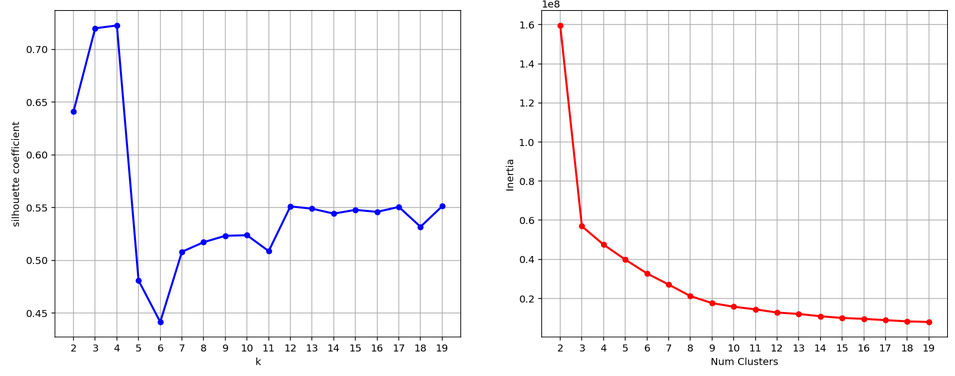
\includegraphics[scale=0.45]{figures/silhouette-elbow-methods}
\centering
\caption{Aplicación de los métodos \textit{Silhouette} (izquierda) y \textit{Elbow} (derecha) para la obtención del número óptimo de clusters.}
\label{fig:silhouette-elbow-methods}
\end{figure}

\begin{figure}[!th]
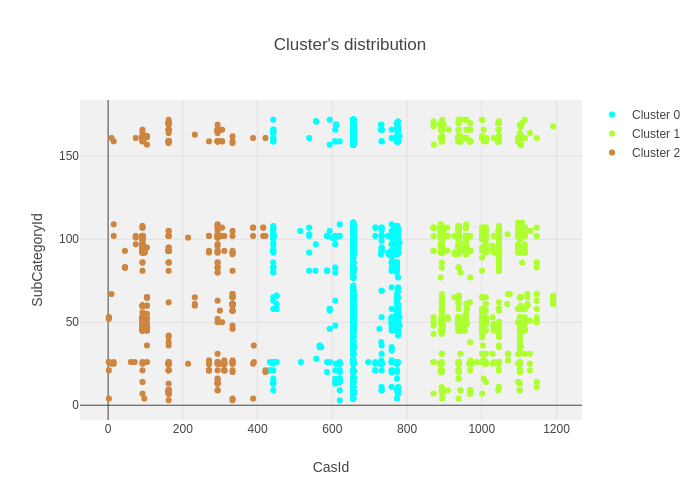
\includegraphics[scale=0.5]{figures/clusters-distribution}
\centering
\caption{Distribución de los clusters según la relación entre los productos químicos \code{CasId} y los cosméticos \code{SubCategoryId}.}
\label{fig:clusters-distribution}
\end{figure}

\begin{table}[!th]
\begin{tabular}{@{}ccc@{}}
\toprule
Cluster 0 & Cluster 1 & Cluster 2 \\ \midrule
5.532 & 1.476 & 479 \\
\bottomrule
\end{tabular}
\centering
\caption{Distribución de los clusters según el número de registros de cada cluster.}
\label{tab:clusters-distribution}
\end{table}



%------------------------------------------------   
\subsection{Métricas del clustering}

Tras aplicar el clustering, se van a calcular ciertas métricas sobre los clusters obtenidos para ofrecer los resultados del clustering de manera más precisa. Las métricas que han sido utilizadas son las siguientes:

\begin{itemize}
 \item \code{Average Within} \citep{metrics}. Mide la distancia media dentro de las observaciones de cada cluster (distancia intra-cluster). Viene definido por la ecuación \ref{eq:average-within}, siendo $K$ el número de clusters, $C_i$ el conjunto de elementos del cluster $i$ y $centroid_i$ el centroide del cluster $i$: 
 \begin{equation}
  SSE = \sum\limits^{K}_{i=1} \sum\limits_{x \in C_i} dist(centroid_i, x)^2
  \label{eq:average-within}
 \end{equation}
 
 \item \code{Dunn Index} \citep{metrics}. Define el ratio entre la distancia mínima inter-cluster y la máxima distancia intra-cluster. Viene definido por la ecuación \ref{eq:dunn-index}, siendo $C$ el conjunto de todos los clusters.
  \begin{equation}
  D(C) = \frac{\min\limits_{C_k, C_l \in C, C_k \neq C_l} (\min\limits_{i,j \in C_k, C_l} dist(i, j))}{\max\limits_{C_m \in C} diam(C_m)}
  \label{eq:dunn-index}
 \end{equation}
\end{itemize}

Así pues, las métricas obtenidas se muestran en la Tabla \ref{tab:metrics}:

\begin{table}[!th]
\begin{tabular}{@{}cc@{}}
\toprule
\code{Average Within} & \code{Dunn Index} \\ \midrule
$0.048633$ & $5.692750 \cdot 10^7$ \\
\bottomrule
\end{tabular}
\centering
\caption{Valores obtenidos para las métricas \code{Average Within} y \code{Dunn Index}.}
\label{tab:metrics}
\end{table}








%------------------------------------------------   
\section{Data Analysis}
\label{sec:results-data-analysis}

El Análisis Exploratorio de Datos \textit{(Exploratory Data Analysis (EDA))} \citep{eda} es muy importante para poder obtener información y conocimiento acerca del dataset. Así pues, en esta sección se van a aplicar distintas técnicas para poder obtener qué productos químicos son los más frecuentes, qué cosméticos son los que presentan mayor número de productos químicos, cómo se distribuyen los datos en función de ciertos campos y cómo se distribuyen por cluster, la cantidad de productos químicos totales. Todo esto se encuentra implementado en el notebook \code{src/clustering-and-data-analysis.ipynb} \citep{master}.



%------------------------------------------------   
\subsection{Obtención de los productos químicos más frecuentes en los cosméticos}
\label{sec:casid-histograms}

La obtención de los productos químicos más frecuentes en los cosméticos se va a realizar realizando histogramas sobre el campo \code{CasId} del dataset. La Figura \ref{fig:histogram-casid-basic} muestra el histograma sobre todo el dataset, donde se puede observar que entre los valores 600 y 700 hay un gran volumen. \\

Concretamente, este volumen se encuentra entre los valores 656 and 658. La Figura \ref{fig:histogram-casid-656-658} muestra el histograma entre dichos valores, donde se puede observar que el volumen se encuentra en el producto químico con \code{CasId} 656, cuyo nombre es: 
\begin{itemize}
 \item \code{656 - Titanium dioxide}.
\end{itemize}

y pertenece al Cluster 0. 

\begin{figure}[!th]
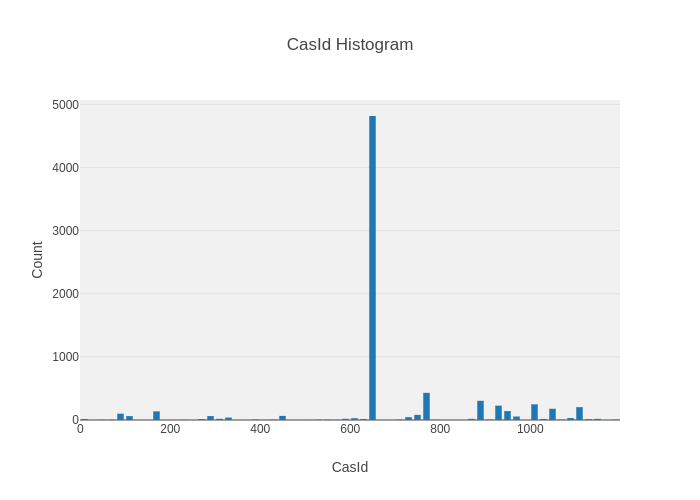
\includegraphics[scale=0.5]{figures/histogram-casid-basic}
\centering
\caption{Histograma sobre el campo \code{CasId}.}
\label{fig:histogram-casid-basic}
\end{figure}

\begin{figure}[!th]
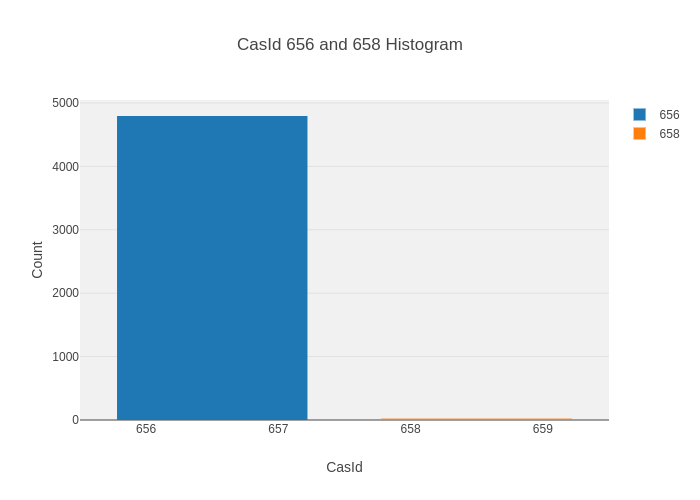
\includegraphics[scale=0.5]{figures/histogram-casid-656-658}
\centering
\caption{Histograma de los valores 656 y 658 del campo \code{CasId}.}
\label{fig:histogram-casid-656-658}
\end{figure}


Sin embargo, como podemos observar en la Figura \ref{fig:histogram-casid-basic}, la diferencia de volumen es muy grande entre el \code{CasId} 656 y el resto. Por lo que se va a realizar los mismos pasos anteriores, pero quitando el \code{CasId} 656 de los datos. \\

La Figura \ref{fig:histogram-casid-without656} muestra el histograma sobre el campo \code{CasId} del dataset sin el \code{CasId} 656 y, además, diferenciando por cluster, donde se puede observar que sigue habiendo un gran volumen entre los valores 700 y 800 y que pertenecen al Cluster 0.


\newpage
\begin{figure}[!th]
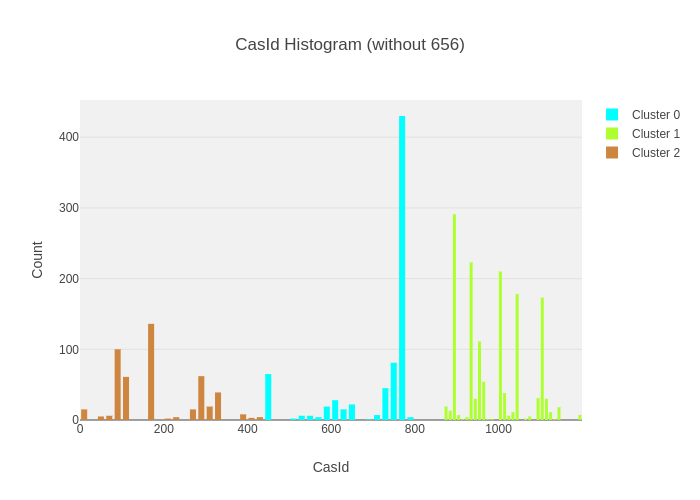
\includegraphics[scale=0.5]{figures/histogram-casid-without656}
\centering
\caption{Histograma sobre el campo \code{CasId} sin el \code{CasId} 656, diferenciando por cluster.}
\label{fig:histogram-casid-without656}
\end{figure}

Concretamente, este volumen se encuentra entre los valores 773 y 776. La Figura \ref{fig:histogram-casid-773-776} muestra el histograma de dichos valores, donde se puede apreciar que el \code{CasId} 773 tiene mayor volumen. El nombre de cada uno de los productos químicos es:

\begin{itemize}
 \item \code{773 - Retinol/retinyl esters, when in daily dosages in excess of 10,000 IU, or 3,000 retinol equivalents}.
 \item \code{776 - Silica, crystalline (airborne particles of respirable size)}.
\end{itemize}


\newpage
\begin{figure}[!th]
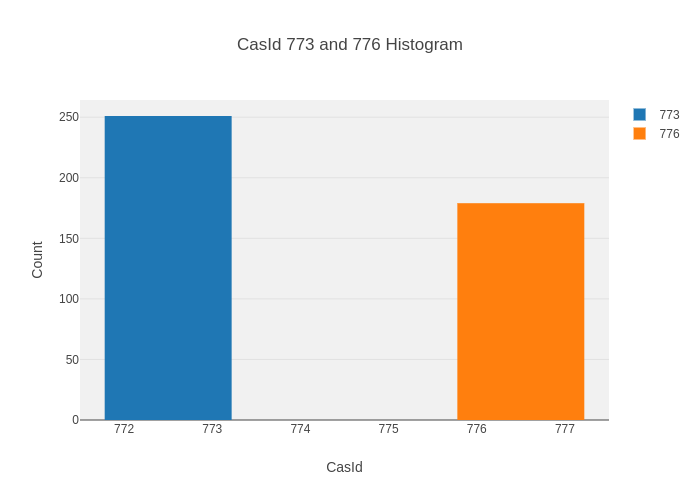
\includegraphics[scale=0.49]{figures/histogram-casid-773-776}
\centering
\caption{Histograma de los valores 773 y 776 del campo \code{CasId}.}
\label{fig:histogram-casid-773-776}
\end{figure}









%------------------------------------------------   
\subsection{Obtención de los cosméticos con mayor número de productos químicos}
\label{sec:subcategoryid-histograms}

Con la misma filosofía que en la sección \ref{sec:casid-histograms}, se van a realizar histogramas sobre el campo \code{SubCategoryId} para obtener los cosméticos que presentan mayor número de productos químicos. La Figura \ref{fig:histogram-subcategoryid-per-cluster} muestra el histograma sobre el campo \code{SubCategoryId} de todo el dataset diferenciando por cluster.

\begin{figure}[!th]
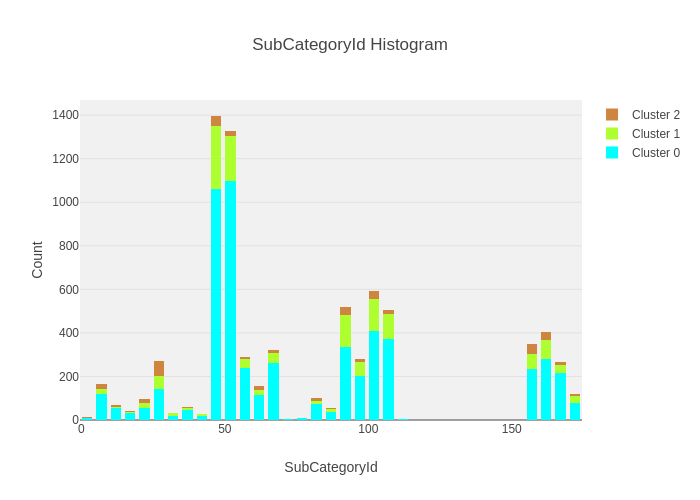
\includegraphics[scale=0.5]{figures/histogram-subcategoryid-per-cluster}
\centering
\caption{Histograma sobre el campo \code{SubCategoryId} diferenciando por cluster.}
\label{fig:histogram-subcategoryid-per-cluster}
\end{figure}


Como se puede observar, hay un gran volumen de registros que pertenecen al Cluster 0, esto es debido al volumen que presenta el \code{CasId} 656 en todo el dataset. Por lo tanto, para poder hacer un estudio más detallado, se va a eliminar el \code{CasId} 656. Así pues, la Figura \ref{fig:histogram-subcategoryid-per-cluster-without656} muestra el mismo histograma que en la Figura \ref{fig:histogram-subcategoryid-per-cluster} pero sin el \code{CasId} 656. 

\begin{figure}[!th]
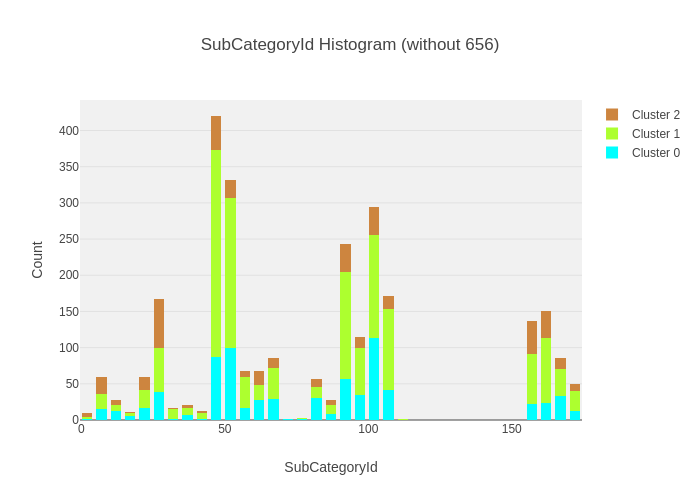
\includegraphics[scale=0.5]{figures/histogram-subcategoryid-per-cluster-without656}
\centering
\caption{Histograma sobre el campo \code{SubCategoryId} diferenciando por cluster, sin el \code{CasId} 656.}
\label{fig:histogram-subcategoryid-per-cluster-without656}
\end{figure}

Al igual que ocurrió con el campo \code{CasId}, se puede observar que entre los valores 40 y 50 del campo \code{SubCategoryId} se encuentra un volumen superior al resto. Concretamente, se encuentra entre los valores 45, 46, 48 y 49. La Figura \ref{fig:histogram-subcategoryid-45-49} muestra el histograma de dichos valores, donde se puede apreciar que el valor \code{SubCategoryId} 48 es el que tiene un volumen mayor. Además, también se puede observar que la gran mayoría de los registros pertenecen al Cluster 1. \\

El nombre de cada uno de los cosméticos es:

\begin{itemize}
 \item \code{45 - Blushes}.
 \item \code{46 - Eyeliner/Eyebrow Pencils}.
 \item \code{48 - Eye Shadow}.
 \item \code{49 - Face Powders}.
\end{itemize}


\newpage
\begin{figure}[!th]
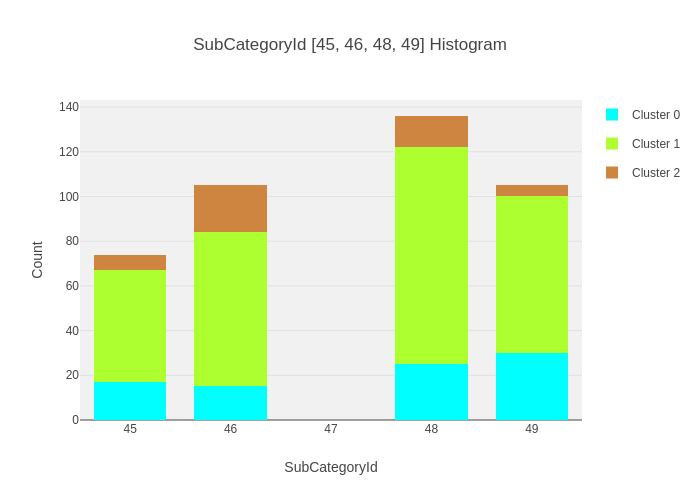
\includegraphics[scale=0.5]{figures/histogram-subcategoryid-45-49}
\centering
\caption{Histograma de los valores 45, 46, 48 y 49 del campo \code{SubCategoryId} diferenciando por cluster, sin el \code{CasId} 656.}
\label{fig:histogram-subcategoryid-45-49}
\end{figure}



\newpage
%------------------------------------------------   
\subsection{Distribución del dataset}
\label{sec:dataset-distribution}

En la Figura \ref{fig:splom-data-aggregated} se muestra la distribución del dataset en función de los campos \code{CasId}, \code{InitialDateReported\_Year}, \code{MostRecentDateReported\_Year} y \code{SubCategoryId}, diferenciando por cluster, en el que se puede observar que en los primeros años (2009 y 2010) fue cuando se reportaron la gran mayoría de los productos químicos y que en los años siguientes han ido reportándose de una manera muy equilibrada.

\begin{figure}[!th]
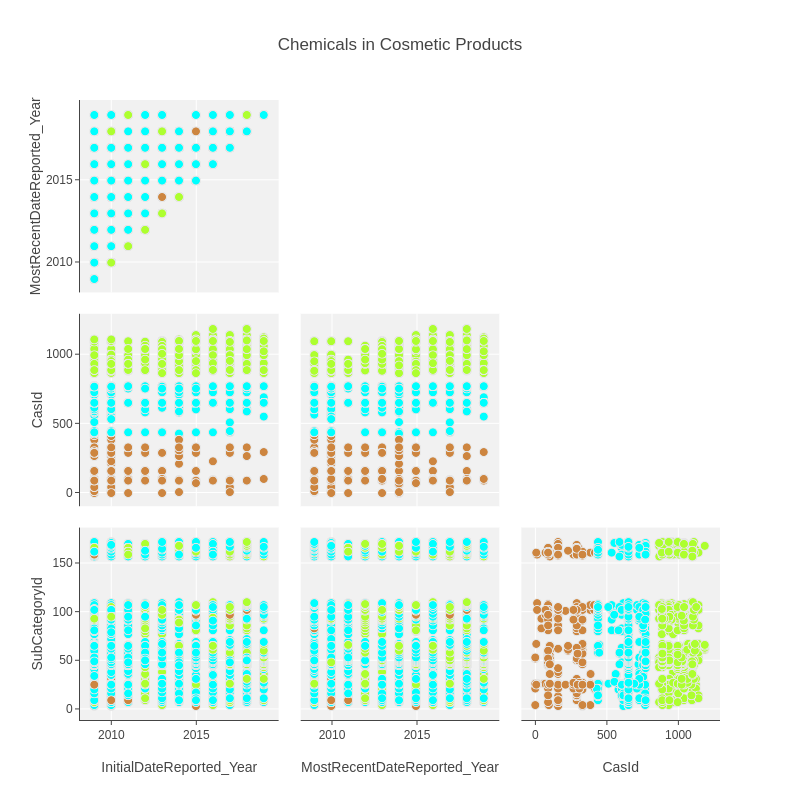
\includegraphics[scale=0.5]{figures/splom-data-aggregated}
\centering
\caption{Distribución del dataset en función de los campos \code{InitialDateReported\_Year}, \code{MostRecentDateReported\_Year}, \code{SubCategoryId} y \code{CasId}.}
\label{fig:splom-data-aggregated}
\end{figure}




\newpage
%------------------------------------------------   
\subsection{Distribución de la cantidad de productos químicos por cluster}
\label{sec:chemicals-per-cluster}

Hasta ahora se han estudiado la frecuencia en la que aparecen los productos químicos y los cosméticos en el dataset. En este punto, se va a estudiar la distribución de la cantidad de productos químicos en cada uno de los clusters, esto es: la suma del campo \code{ChemicalCount} distribuido en cada uno de los clusters. La Figura \ref{fig:pie-sum-chemicalcount} muestra esta distribución.


\begin{figure}[!th]
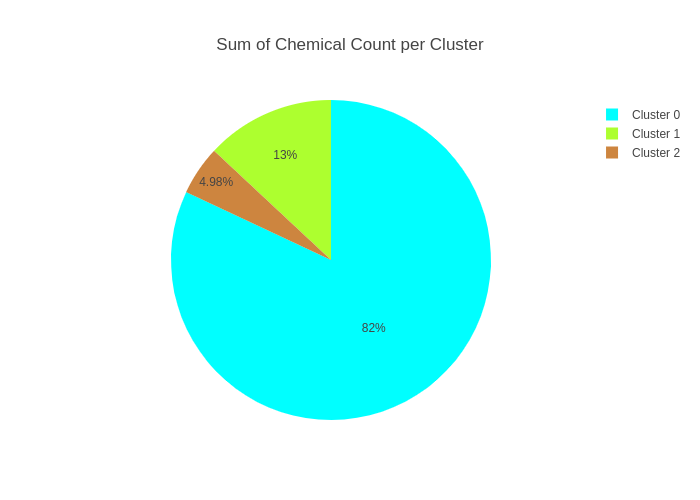
\includegraphics[scale=0.46]{figures/pie-sum-chemicalcount}
\centering
\caption{Distribución de la suma del campo \code{ChemicalCount} por cada cluster.}
\label{fig:pie-sum-chemicalcount}
\end{figure}

Al igual que pasaba en la sección \ref{sec:subcategoryid-histograms}, el alto porcentaje del Cluster 0 se debe al \code{CasId} 656. Por lo que, la Figura \ref{fig:pie-sum-chemicalcount-without656} muestra la misma distribución eliminando el \code{CasId} 656 del dataset. Donde se puede observar que más del 50\% de los productos químicos se encuentran en el Cluster 1.

\begin{figure}[!th]
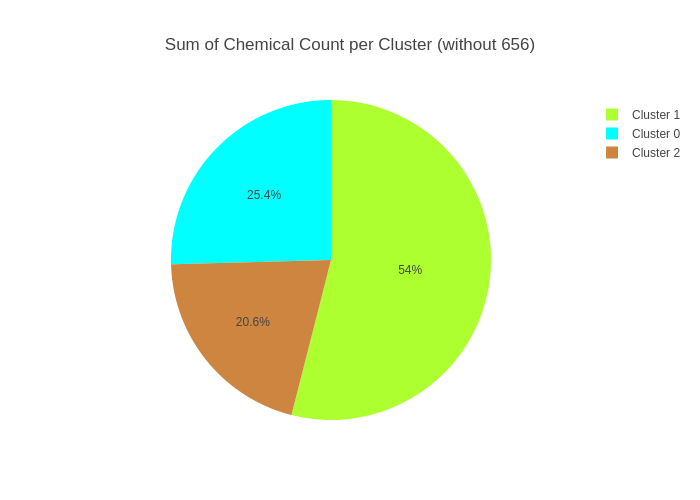
\includegraphics[scale=0.46]{figures/pie-sum-chemicalcount-without656}
\centering
\caption{Distribución de la suma del campo \code{ChemicalCount} por cada cluster, sin el \code{CasId} 656.}
\label{fig:pie-sum-chemicalcount-without656}
\end{figure}

\newpage

%------------------------------------------------   
\section{Forecasting}





%------------------------------------------------   
\subsection{Preprocesamiento}

Antes de poder aplicar el algoritmo de forecasting ARIMA \citep{arima}, el dataset debe ser preprocesado, al igual que se realizó con el clustering en la sección \ref{sec:clustering-preprocessing}. Sin embargo, no se ha realizado el mismo preprocesamiento. A continuación se detallan los pasos realizados en este preprocesamiento:

\begin{itemize}
 \item \textbf{Rellenar valores nulos}. En el dataset se han encontrado tres tipos de valores nulos: 
 \begin{itemize}
  \item \textbf{Valores de formato fecha}. Han sido rellenados con el valor \code{01/01/1990}.
  \item \textbf{Valores de formato texto}. Han sido rellenados con el valor de la cadena vacía.
  \item \textbf{Valores de formato texto asociados a identificadores}. Han sido rellenados con el valor \code{-1}.
 \end{itemize}
 
 \item \textbf{Eliminar de los registros} con valor distinto de \code{01/01/1990} en los campos \\ \code{DiscontinuedDate} y \code{ChemicalDateRemoved}, pues solo se precisan de aquellos registros de cosméticos que tengan productos químicos y no hayan sido retirados del mercado.

 \item \textbf{Agrupar por el campo} \code{InitialDateReported} sumando los valores del campo \\ \code{ChemicalCount}. Ya que el objetivo de la aplicación de forecasting es poder obtener una predicción de la cantidad de productos químicos que serán reportados en el futuro.
\end{itemize}

Tras aplicar este preprocesamiento nos queda un dataset con 1.863 registros y 2 características: \code{InitialDateReported} y \code{ChemicalCount}.




%------------------------------------------------   
\subsection{Obtención de los datasets de entrenamiento y validación}


Para poder realizar el forecasting, se necesita tener datos de entrenamiento y datos de validación (en adelante, \code{dataset} y \code{validation}, respectivamente). La obtención de estos datasets está ligada a que el dataset \citep{dataset} es incremental y se tienen almacenados dos versiones del dataset, como se ha comentado en la sección \ref{sec:data-downloading}. \\ 

Así, se disponen de las siguientes versiones del dataset:

\begin{itemize}
 \item Carpeta \code{src/data/} \citep{master}, donde se almacena la versión más reciente del dataset.
 \item Carpeta \code{src/data\_backup/} \citep{master}, donde se almacena la versión anterior del dataset.
\end{itemize}












\newpage
%------------------------------------------------   
\subsection{Aplicación del algoritmo ARIMA}


















% Chapter Template

\chapter{Discusión} % Main chapter title
\label{chap:discussion} % Change X to a consecutive number; for referencing this chapter elsewhere, use \ref{ChapterX}


%------------------------------------------------   
\section{Introducción}

En este capítulo se analizarán los resultados obtenidos en el capítulo \ref{chap:results} y se discutirá acerca de los modelos obtenidos. Primero, se analizarán los resultados obtenidos tras la aplicación del clustering y, posteriormente, los obtenidos tras la aplicación del forecasting.






%------------------------------------------------   
\section{Clustering}

La aplicación del algoritmo de clustering K-Means \citep{scikit-learn} sobre el dataset \citep{dataset} que se ha realizado en la sección \ref{sec:results-clustering} ha proporcionado la siguiente información:

\begin{itemize}
 \item El dataset se divide en 3 clusters, cuya distribución se muestra en la Figura \ref{fig:clusters-distribution} de manera gráfica y en la Tabla \ref{tab:clusters-distribution} de manera numérica.
 
 \item La diferencia de volumen entre el Cluster 0 y el resto de clusters es debido a que en el Cluster 0 se encuentra el \code{CasId} 656, que es el producto químico más frecuente en todo el dataset, como se comenta en la sección \ref{sec:results-data-analysis}.

 \item Las métricas obtenidas sobre los clusters que muestra la Tabla \ref{tab:metrics} indican que los clusters están muy juntos (métrica \code{Dunn Index}) y que el tamaño de los mismos es muy grande (métrica \code{Average Within}), lo que concuerda con la distribución mostrada en la Figura \ref{fig:clusters-distribution}.
\end{itemize}

Con esta información, se puede concluir que la clusterización obtenida es la óptima para este dataset.





%------------------------------------------------   
\section{Forecasting}

La aplicación del algoritmo de forecasting ARIMA \citep{arima} sobre el dataset \citep{dataset} que se ha realizado en la sección \ref{sec:results-forecasting} ha proporcionado la siguiente información:

\begin{itemize}
 \item Se han obtenido cuatro modelos ARIMA para cuatro agrupaciones distintas del dataset: agrupando por mes (\code{by\_month}), agrupando cada 15 días (\code{by\_each\_15days}), agrupando cada 7 días (\code{by\_each\_7days}) y sin agrupación (\code{alldataset}). La Tabla \ref{tab:ts-model-comparation} resume los valores obtenidos por cada uno de los modelos.
 
\begin{table}[!th]
\begin{tabular}{@{}cccccc@{}}
\toprule
Modelo                  & \code{(p,d,q)} & \code{dataset} & $RMSE_{dataset}$ & \code{validation} & $RMSE_{validation}$ \\ \midrule
\code{by\_month}        & (1,1,0)        & 110                   & 18.822           & 6                        & 15.212 \\
\code{by\_each\_15days} & (1,1,0)        & 223                   & 15.903           & 12                       & 19.856 \\
\code{by\_each\_7days}  & (1,1,0)        & 467                   & 15.064           & 25                       & 17.986 \\
\code{alldataset}       & (1,1,0)        & 1.749                 & 12.905           & 114                      & 23.571 \\
\bottomrule
\end{tabular}
\centering
\caption{Resumen de los valores obtenidos por los cuatro modelos ARIMA.}
\label{tab:ts-model-comparation}
\end{table}


 \item Como se puede observar, conforme el tamaño del dataset de entrenamiento \code{dataset} aumenta, el RMSE disminuye, mientras que conforme el tamaño del dataset de validación \code{validation} aumenta, el RMSE aumenta, exceptuando en el dataset obtenido agrupando cada 7 días (\code{by\_each\_7days}).
 
 \item El modelo obtenido a partir de todo el dataset (\code{alldataset}) tiene un RMSE muy pequeño en comparación con el tamaño del dataset, por lo que el mejor modelo a aplicar sería este. Sin embargo, poder predecir la cantidad de productos químicos que habrá en un día en concreto no es tan relevante como poder predecir la cantidad de productos químicos que habrá cada semana o cada dos semanas.
 
 \item Así pues, con estas características, el modelo que mejor se ajusta es el modelo a partir de la agrupación del dataset cada 7 días (\code{by\_each\_7days}).

\end{itemize}




















% Chapter Template

\chapter{Conclusiones} % Main chapter title
\label{chap:conclusions} % Change X to a consecutive number; for referencing this chapter elsewhere, use \ref{ChapterX}


%------------------------------------------------   
\section{Conclusiones del trabajo}

La realización de este Trabajo Fin de Master ha dado como resultado la consecución de los objetivos marcados en la sección \ref{sec:goals}:

\begin{itemize}
 \item Se ha implementado un modelo de clustering que clasifica los productos químicos presentes en los cosméticos en 3 grandes grupos: Cluster 0, Cluster 1 y Cluster 2.
 
 \item Se ha obtenido un modelo de forecasting capaz de predecir la cantidad de productos químicos presentes en los cosméticos en un periodo de una semana.
 
 \item Se han encontrado los productos químicos más frecuentes en los cosméticos:
\begin{itemize}
  \item \code{656 - Titanium dioxide}.
  \item \code{773 - Retinol/retinyl esters, when in daily dosages in \\ excess of 10,000 IU, or 3,000 retinol equivalents}.
  \item \code{776 - Silica, crystalline (airborne particles of \\ respirable size)}.
 \end{itemize}

 siendo \code{656 - Titanium dioxide} el más frecuente en todo el dataset.
 
 \item Se han encontrado los cosméticos con mayor presencia de productos químicos (sin tener en cuenta el \code{656 - Titanium dioxide}):
 \begin{itemize}
  \item \code{45 - Blushes}.
  \item \code{46 - Eyeliner/Eyebrow Pencils}.
  \item \code{48 - Eye Shadow}.
  \item \code{49 - Face Powders}.
 \end{itemize}
 
 siendo \code{48 - Eye Shadow} el cosmético con mayor presencia de productos químicos entre ellos.
 
 \item Y se ha encontrado que más del 80\% de la cantidad de productos químicos se encuentran dentro del Cluster 0, teniendo en cuenta que en este cluster se encuentra el \code{656 - Titanium dioxide}. Sin este producto químico, más del 50\% de la cantidad de productos químicos se encuentran dentro del Cluster 1. 
\end{itemize}




\newpage
%------------------------------------------------   
\section{Conclusiones personales}

Dada mi inquietud por poder aplicar la informática al campo de la salud, sabía que mi Trabajo Fin de Máster iba a ser una de esas aplicaciones. Sin embargo, no sabía sobre qué tema enfocarlo. Hasta que mi tutor Juan Manuel me descubrió la plataforma HealthData \citep{healthdata} y pude investigar en la inmensidad de datasets públicos en el ámbito de la salud. \\

De todos los datasets que hay en esta plataforma, decidí escoger el dataset \tabhead{Chemicals in Cosmetics} \citep{dataset} porque almacena información muy importante en una actualidad donde el consumo de cosméticos es increíblemente alto, donde algunos cosméticos son casi imprescindibles hoy día. Y el hecho de que los cosméticos contengan productos químicos dañinos para las personas, conlleva a estudiarlos muy a fondo. \\

Además, este dataset me suponía tres retos, todos ligados a la aplicación de técnicas descritas en el capítulo \ref{chap:results}: 

\begin{itemize}
 \item ¿Cómo obtengo el dataset si se va actualizando cada cierto tiempo?
 \item ¿Cómo aplico el clustering sobre un dataset tan grande?
 \item ¿Cómo se aplican las técnicas de forecasting? y ¿cómo aplico el forecasting sobre un dataset incremental?
\end{itemize}

La realización de este Trabajo Fin de Máster es el fruto de la consecución de los tres retos anteriores. Tal vez este trabajo no llegue a ser nada más que un simple Trabajo Fin de Máster, que se quedará en el recuerdo, pero yo me siento orgulloso de volver a poner mi granito de arena sobre la aplicación de la informática al campo de la salud.




























%----------------------------------------------------------------------------------------
%	THESIS CONTENT - APPENDICES
%----------------------------------------------------------------------------------------

\appendix % Cue to tell LaTeX that the following "chapters" are Appendices

% Include the appendices of the thesis as separate files from the Appendices folder
% Uncomment the lines as you write the Appendices

% \include{appendices/file-format}
% \include{appendices/user-manual}

%----------------------------------------------------------------------------------------
%	GLOSSARY
%----------------------------------------------------------------------------------------
% \printglossary[type=glossary]

%----------------------------------------------------------------------------------------
%	BIBLIOGRAPHY
%----------------------------------------------------------------------------------------
\bibliography{bib}

%----------------------------------------------------------------------------------------

\end{document}  
